\documentclass[11pt]{article}
\usepackage{graphicx}
\usepackage{hyperref}
\usepackage{caption}



\newcommand{\numpy}{{\tt numpy}}    % tt font for numpy

\topmargin -.5in
\textheight 9in
\oddsidemargin -.25in
\evensidemargin -.25in
\textwidth 7in

\begin{document}

% ========== Edit your name here
\author{Due by 5:00pm Friday, February 11 2022}
\title{CS 498: Assignment 1: Perspective Projection}
\date{January 28, 2022}
\maketitle

\medskip


\section*{Submission}

In this assignment you will be modifying the files homography.py perspective.py.
Please put together a single PDF with your answers and figures for each problem, and submit to Gradescope (Course Code: JBXJVZ). We recommend you to add your answers to the latex template files we provided. For code submission, make sure you use the provided ".py" files with your modification and the dumped ``.npz'' file. The graders will check both your PDF submission and your code submission if needed. 


\section*{Homography [8pts]}

In this question, we will examine properties of homography transformations and see how to estimate a planar homography from a set of correspondences. 

\paragraph{Question 1 [1pt]:} You are given a photo of the State Farm Center (\texttt{uiuc.png}), UIUC's indoor arena that hosts our basketball teams. We marked and plotted the four corners of the court, as shown in Fig.~\ref{fig:intro} (left). A standard basketball court is 28.65 meters long and 15.24 meters wide, as shown in Fig.~\ref{fig:intro} (right). Now let's consider a 2D coordinate system defined on the planar surface of the basketball court. The origin of this coordinate system is point \#3; the long edge is x axis and short edge is y axis. Please write down the four corner's coordinate in this 2D coordinate frame (in meters) and fill in your answer in the numpy array "corners\_court". 

\begin{figure}[htbp]
\small
\includegraphics[width=0.48\linewidth]{goillini.png}
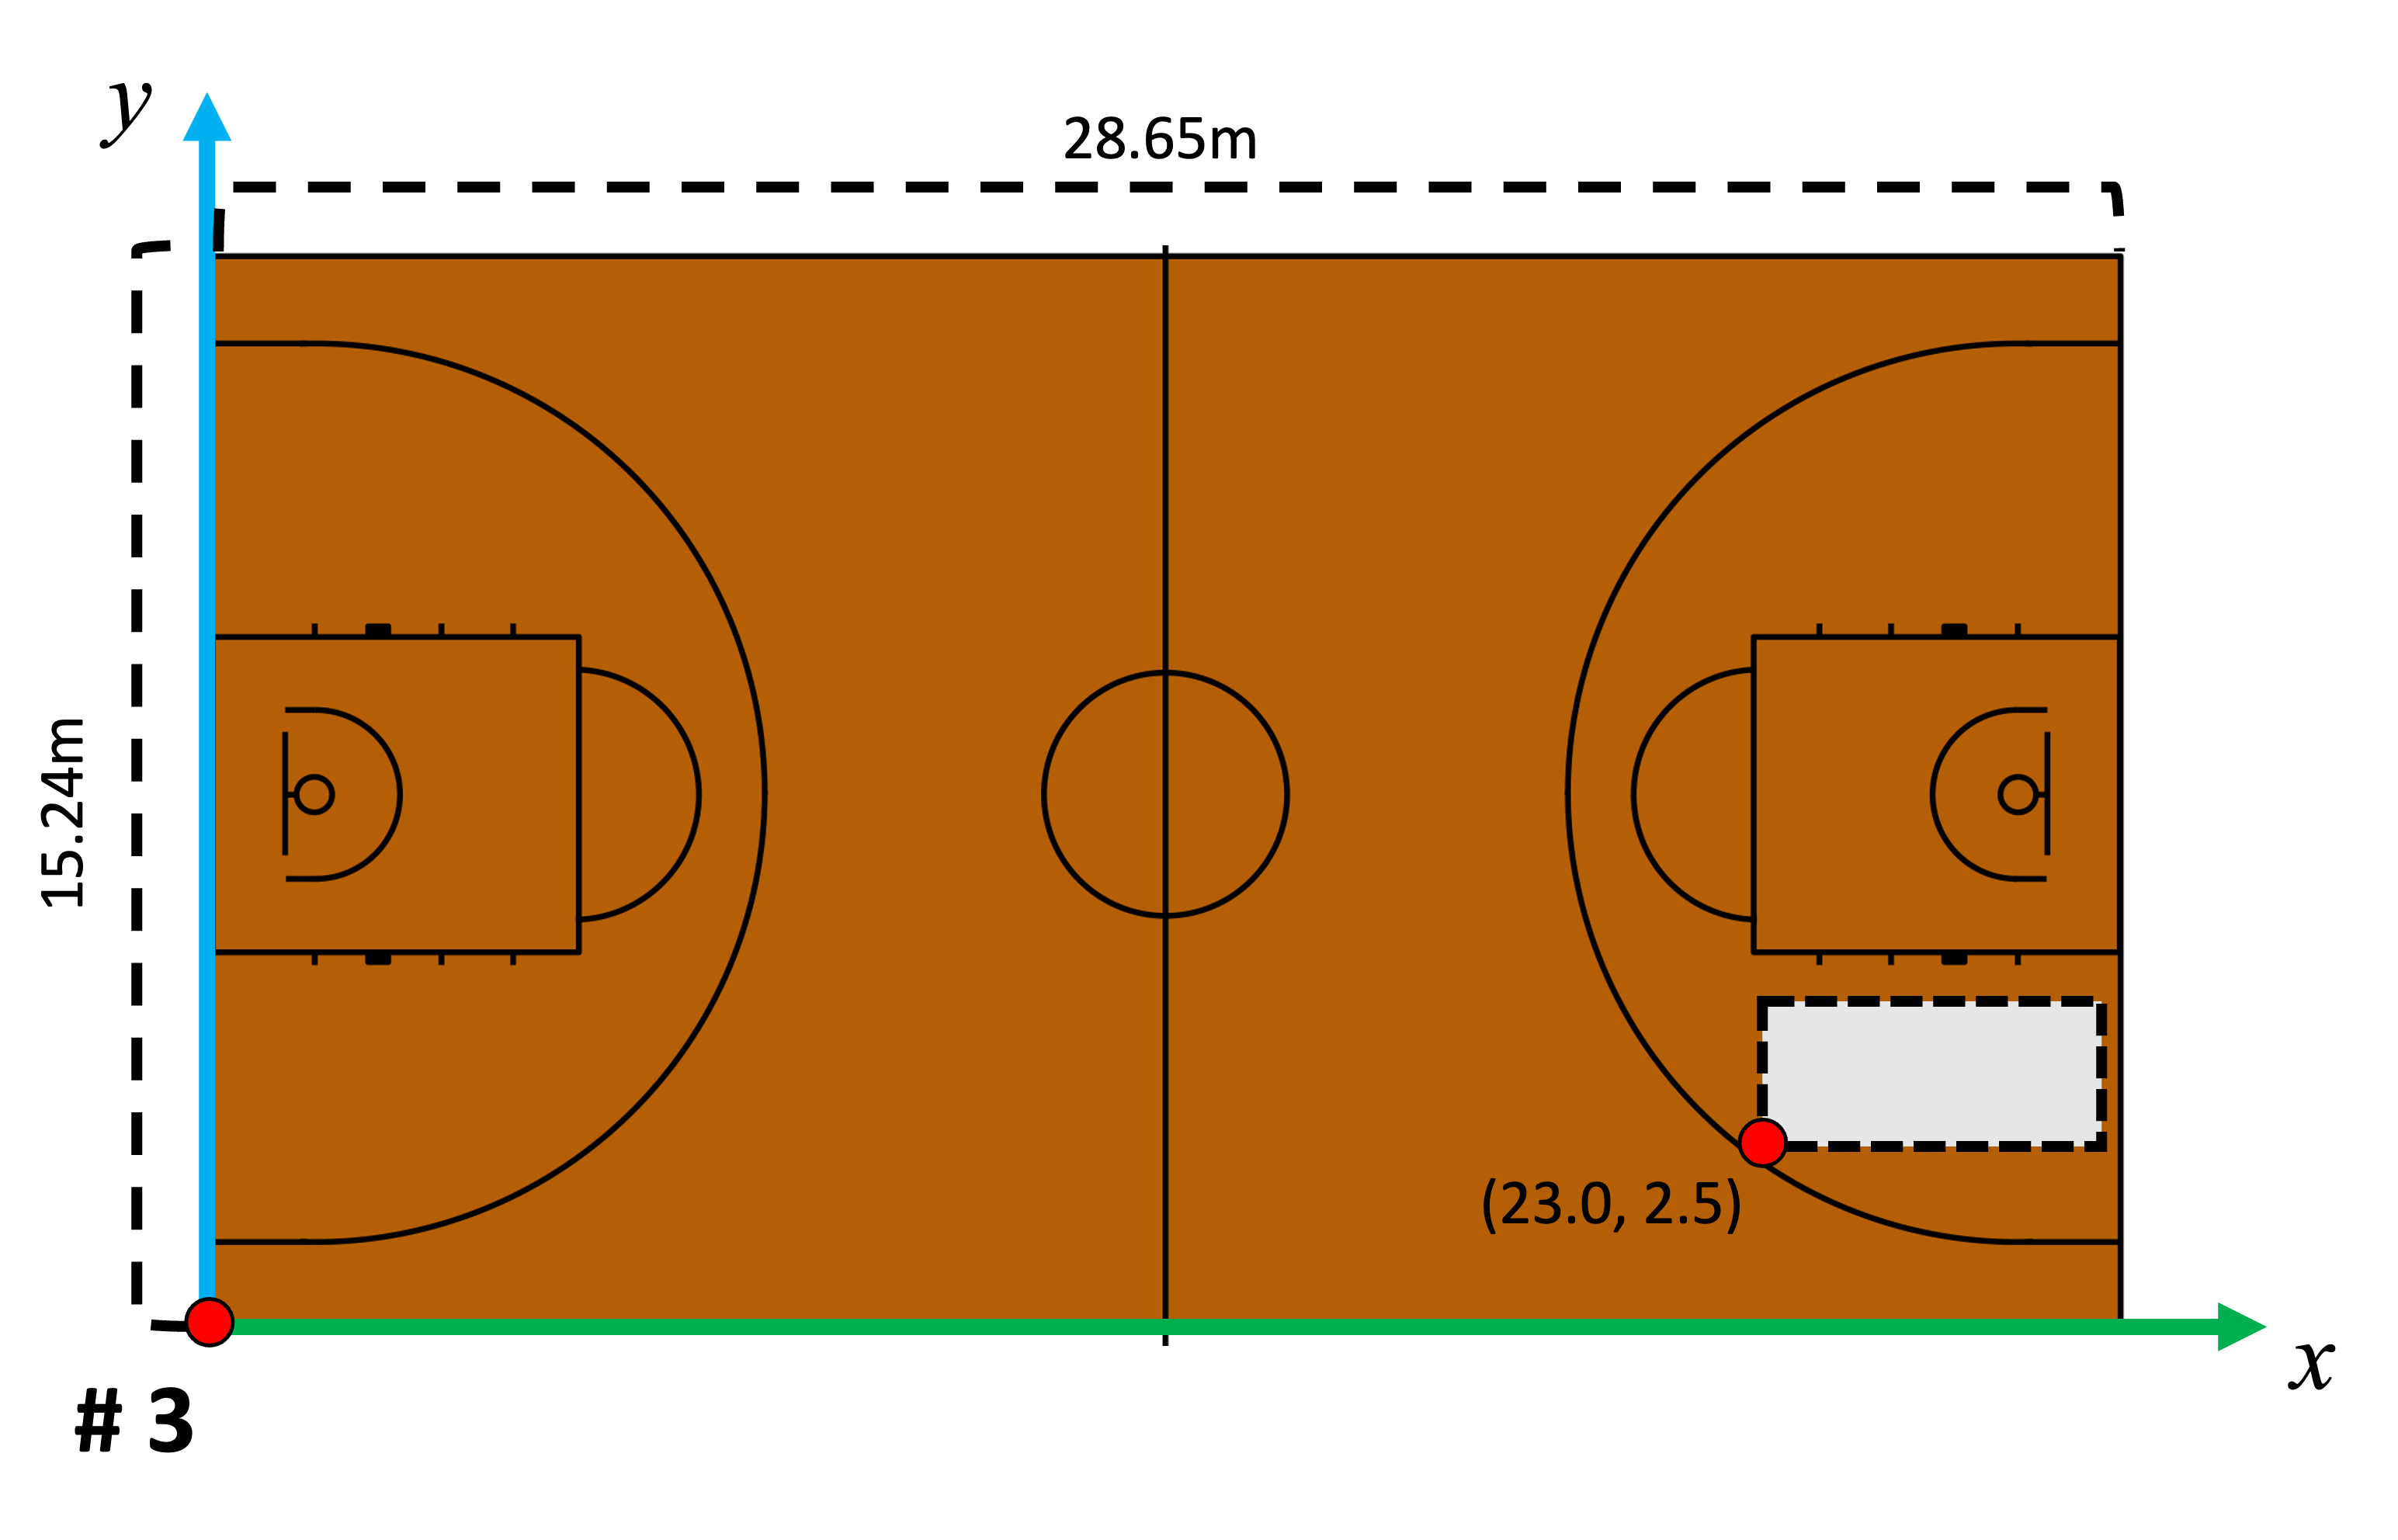
\includegraphics[width=0.5\linewidth]{coordinate.png}
\caption{ Left: target image with keypoints; Right: court dimensions and coordinate convention.}
\label{fig:intro}
\end{figure}


\paragraph{Question 2 [3pts]:}
Given your Q1's answer, now we could establish four pairs of point correspondence between two planes: the 2D basketball court plane and the 2D image plane. Using what we have learned in Lecture 3, complete the function \texttt{findHomography} and use it to estimate the homography matrix from the court to the image. Please briefly explain what you do for homography estimation and report the resulting matrix in this document. Hints: 1) you might find the function \texttt{vstack, hstack} to be handy for getting homogenous coordinate; 2) you might find \texttt{numpy.linalg.svd} to be useful; 3) lecture 3 described the homography estimate process. 

% \[
% \left[
% \begin{array}{c}
% x \\
% y \\
% z
% \end{array}
% \right] = 
% \left[
% \begin{array}{cccc}
% p_1 & p_2 & p_3 & p_4 \\
% p_5 & p_6 & p_7 & p_8 \\
% p_9 & p_{10} & p_{11} & p_{12} \\
% \end{array}
% \right]
% \left[
% \begin{array}{c}
% X \\
% Y \\
% Z \\
% 1
% \end{array}
% \right]
% \]

% \[
% \left[
% \begin{array}{ccccccccc}
% 0 & 0 & 0 & X_1 & Y_1 & 1 & -y_1^\prime X_1 & -y_1^\prime Y_1 & -y_1^\prime \\
% X_1 & Y_1 & 1 & 0 & 0 & 0 & -x_1^\prime X_1 & -x_1^\prime Y_1 & -x_1^\prime \\
% 0 & 0 & 0 & X_2 & Y_2 & 1 & -y_2^\prime X_2 & -y_2^\prime Y_2 & -y_2^\prime \\
% X_2 & Y_2 & 1 & 0 & 0 & 0 & -x_2^\prime X_2 & -x_2^\prime Y_2 & -x_2^\prime \\
% 0 & 0 & 0 & X_3 & Y_3 & 1 & -y_3^\prime X_3 & -y_3^\prime Y_3 & -y_3^\prime \\
% X_3 & Y_3 & 1 & 0 & 0 & 0 & -x_3^\prime X_3 & -x_3^\prime Y_3 & -x_3^\prime \\
% 0 & 0 & 0 & X_4 & Y_4 & 1 & -y_4^\prime X_4 & -y_4^\prime Y_4 & -y_4^\prime \\
% X_4 & Y_4 & 1 & 0 & 0 & 0 & -x_4^\prime X_4 & -x_4^\prime Y_4 & -x_4^\prime \\
% \end{array}
% \right]
% \left[
% \begin{array}{c}
% h_1 \\
% h_2 \\
% h_3 \\
% h_4 \\
% h_5 \\
% h_6 \\
% h_7 \\
% h_8 \\
% h_9
% \end{array}
% \right] = \mathbf{0}
% \]



\paragraph{Question 3 [4pts]:}

We want to promote our CS498 class across the university. One of the marketing idea we came up is to create an on-court ad in Illinois's State Farm Center. Now you are taking in charge of the virtual signage task --  inserting the logo of our class (\texttt{logo.png}) electronically onto the basketball court (\texttt{court.png}). Specifically, the size of the logo needs to be 3x6 meters; we want to place the bottom left logo corner at $(23, 2)$ on the basketball court. In order to do so, we need two steps: 

\begin{itemize}
\item \textbf{3.a [1pt]:} calculate the homography transform between the image coordinate of the two images \texttt{logo.png} and \texttt{court.png}. Hints: 1) could you compute the transform from \texttt{logo.png} to the basketball court 2) could you leverage the homography matrix you computed in Question 2? 
\item \textbf{3.b [2pt]:} complete the \texttt{warpImage} function and use the homography you computed in 3.a to warp the image \texttt{logo.png} from its image coordinate to the \texttt{court.png}'s image coordinate. Hints: 1) suppose $(x^\prime, y^\prime, 1)^T = \mathbf{H} (x, y, 1)^T$, we have $I_\mathrm{target}(x^\prime, y^\prime) = I_\mathrm{source}(x, y)$; 2) you might find \texttt{numpy.meshgrid} and \texttt{numpy.ravel\_multi\_index} to be useful. 
\item \textbf{3.c [1pt]:} alpha-blend the warped logo onto the court: $I = \alpha F + (1 - \alpha) B$
\end{itemize}



\section*{Perspective Projection [7pts]}
Till now we have been working on transformations between 2D coordinate systems. Now let us to lift up to the 3D coordinate. Consider the same image of the state farm center, but this time, we annotate four additional points, corresponding to the four corners of the basketball backboard. 

\paragraph{Question 4 [1pt]:} 
The lower rim of the backboard is 2.745 meters above the ground; the backboard width is 1.83 meters and backboard height is 1.22 meters. The backboard protrudes 1.22 meters out from the baseline. Now let us consider the world frame. The world frame coordinate origin is at the point \#3, where x-axis is along the long edge (sideline) and y-axis is along the short edge (baseline), and z-axis is upwards, perpendicular to the basketball court.   Could you compute the 3D coordinate of all the eight keypoints?

\paragraph{Question 5 [4pt]:} 
Now we have established eight pairs of 2D and 3D keypoint correspondences. 
Consider this set of correspondence pairs in homogeneous coordinate $(\mathbf{x}_i, \mathbf{X}_i)$. Our goal is to compute a perspective projection matrix such that: 
\[
\mathbf{x}_i = \alpha \mathbf{P} \mathbf{X}_i = 
\alpha \left[
\begin{array}{c}
\mathbf{p}_1^T \\
\mathbf{p}_2^T \\
\mathbf{p}_3^T
\end{array}
\right]
\mathbf{X}_i
= 
\alpha \left[
\begin{array}{c}
\mathbf{p}_1^T\mathbf{X}_i \\
\mathbf{p}_2^T\mathbf{X}_i \\
\mathbf{p}_3^T\mathbf{X}_i
\end{array}
\right]
\]
where $\mathbf{p}_i^T$ is $i$th row of $\mathbf{P}$; $\mathbf{x}_i = (x_i, y_i, 1)^T$; $\alpha$ is an arbitrary scalar. 

\begin{itemize}
\item \textbf{5.a [1pt]:} Please prove that:
\[
\mathbf{A}_i 
\left[
\begin{array}{c}
\mathbf{p}_1^T \\
\mathbf{p}_2^T \\
\mathbf{p}_3^T
\end{array}
\right] = \mathbf{0} \textrm{\ where \ } \mathbf{A}_i = \left[
\begin{array}{ccc}
\mathbf{0} & -\mathbf{X}_i & - y_i \mathbf{X}_i \\
\mathbf{X}_i & \mathbf{0} & - x_i \mathbf{X}_i\\
\end{array}
\right]
\]
Hints: consider using cross product between two similar vectors. 
\item \textbf{5.b [3pt]:} complete the \texttt{findProjection} function and use this function to recover the perspective camera projection matrix, from the 3D world coordinate to the 2D image coordinate. Hints: 1) establish a linear system based on your derivation 2) given the eight keypoint correspondences, how many equations and how many unknown variables? 3) consider using \texttt{numpy.linalg.svd} to solve the linear system. 4) you might find \texttt{numpy.concatenate} and \texttt{numpy.reshape} to be handy.  
\item \textbf{5.c [1pt bonus]:} Try to answer the following questions: 1) assuming perfect correspondences, could we recover the projection matrix using even fewer points? Please indicate how many correspondences at least we need. 2) could we just use correspondences on the ground plane to recover this projection matrix? Please explain why or why not.     
\end{itemize}

\paragraph{Question 6 [2pt]:}
Using our estimated projection matrix in Q5, we could insert any 3D object in the world coordinate frame onto the 2D image. In this question, let's consider the a simple case where we want to project a 3D point cloud onto the image plane and plot them. Suppose we want to put a giant stanford bunny statue in the center of the basketball court, could you compute the 2D coordinate of every vertex of this bunny using the projection matrix? Hints: 1) you might need to transform the bunny to the court center first 2) make sure the bunny is above the ground. 

\paragraph{Question 7 [2pt bonus]:} Try to use an off-the-shelf renderer to render the 3D mesh in a more realistic manner (e.g. pyrender, moderngl, blender, mitsuba2). You could consider the following perspectives that might influence the realism: 1) shading 2) shadows 3) occlusion reasoning 4) lighting environments. 


\end{document}
\grid
\grid